\section{Aufgabe 4}
Das Vorgehen in Aufgabe 4 ist völlig identisch zu dem in Aufgabe 1-3, mit dem Unterschied, dass eine Neonröhre verwendet wird, statt einer Quecksilberröhre. Der Aufbau, Durchführung und Fehlerrechnung können aus den vorherigen Aufgaben übernommen werden.
\subsection{Graphen/Messwerte}
Die Messwerte wurden wieder exportiert und mit GNU-Plot aufgetragen, die Minimalstellen wurden mit dem Auge geschätzt.
\begin{center}
\begin{minipage}{\linewidth}
\centering
\makebox[0cm]{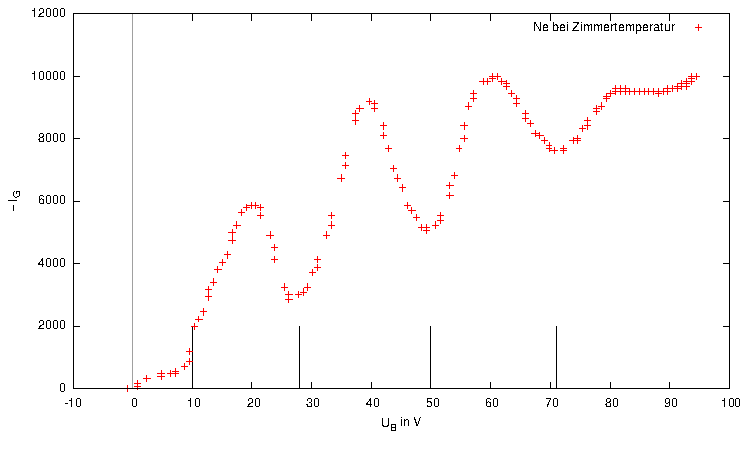
\includegraphics[width=\textwidth]{graphen/a3/a3}}
\captionof{figure}{Franck-Hertz-Kurve von Neon}
\label{a3}
\end{minipage}
\end{center}
Die so gefunden Spannungen \(U_B\) der Minima werden nun tabellarisch und anschließend mit einer linearen Regression dargestellt, um die Steigung \(b\) des als linear angenommen Verlaufs zu erhalten.
\begin{center}
\begin{tabular}{c|c}
Minimum & \(U_B\)\\\hline
\(0\) & \(10\, V\)\\
\(1\) & \(28\, V\)\\
\(2\) & \(50\, V\)\\
\(3\) & \(71\, V\)\\
\end{tabular}
\captionof{table}{Minima von \(U_B\) der aufgenommenen Franck-Hertz-Kurven von Neon}
\end{center}
\begin{center}
\begin{minipage}{\linewidth}
\centering
\makebox[0cm]{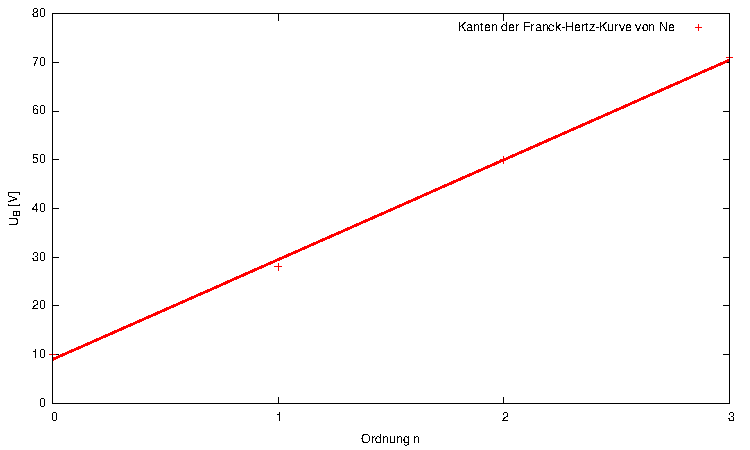
\includegraphics[width=\textwidth]{graphen/a3/graph}}
\captionof{figure}{Minima der Franck-Hertz-Kurve von Neon}
\label{graph_a3}
\end{minipage}
\end{center}
Die Steigung wurde ermittelt zu:
\begin{align}
b = \left( 20,50 \pm 0,59 \right)\, V \notag
\end{align}
\subsection{Auswertung}
Auch die Auswertung läuft wieder völlig analog zu den Aufgaben 1-3.
Die Steigung \(b\) kann also wieder wie in \eqref{E_kin} direkt in eine Energie übersetzt werden, daher gilt für die Anregungsenergie von Neon:
\begin{align}
E = \left( 20,50 \pm 0,59 \right)\, eV \notag
\end{align}
\subsection{Zwischenfazit}
Neon ist bei Zimmertemperatur gasförmig und es wird daher keine weitere Heizung benötigt um den Abstand der Atome hinreichend zu vergrößern. Die ermittelte Anregungsenergie von \(\left( 20,5 \pm 0,6\right)\, eV \) ist identisch zum Literaturwert von \(\left( 18,7 \pm 0,3\right)\, eV \), da die Fehlerintervalle überlappen. Bei Neon geht der Zustand über diverse Nebenzustände zurück in den Grundzustand, weswegen auch ein größeres Intervall für die Anregungsenergie angegeben wird. Beim zurückfallen in den Grundzustand wird auch unter anderem das sichtbare rote Licht emittiert.